\documentclass[../book.tex]{subfiles}

\textbackslash{}chapter\{Patterns and differences \label{ch:pattern}

\begin{quote}
The notion of pattern involves the concept of different modes of
togetherness \autocite[195-6]{Whitehead_1956}.
\index{Whitehead, Alfred North!on pattern}
\index{pattern!modes of togetherness}
\end{quote}

\begin{quote}
Algorithms for pattern recognition were therefore from the very
beginning associated with the construction of linear decision surfaces
\autocite[273-4]{Cortes_1995}
\index{Cortes, Corinna!on pattern recognition}
\end{quote}

Do machine learners generate new patterns of difference? Should we hold
machine learners accountable for their claims to recognise patterns in
data in the same way we hold experimental scientists accountable for
their factual claims?\footnote{Many authors have suggested that
  algorithms should be the focus of more attention. The sociologist Mike
  Savage, in his account of the growth of `descriptive assemblages'
  based around large scale data mining of transactions, administrative
  records and social media practice concludes:

  It follows that a core concern might be to scrutinize how pattern is
  derived and produced in social inscription devices, as a means of
  considering the robustness of such derivations, what may be left out
  or made invisible from them, and so forth. We need to develop an
  account which seeks to criticize notions of the descriptive insofar as
  this involves the simple generation of categories and groups, and
  instead focus on the fluid and intensive generation of potential
  \autocite[171]{Savage_2009}
  \index{Savage, Mike!on descriptive assemblage}}
\index{machine learner!pattern recognition|seealso{pattern}} This
chapter explores two major machine learning treatments of pattern dating
from the last decades of the twentieth century from the standpoint of
differences. I suggest that what counts as pattern changes in machine
learning over time. While much machine learning strains to identify
differences in terms of differences of degree, the practice of
pattern-finding itself harbours differences of kind.
\index{differences!kind versus degree} For critical thought, the
connection between pattern and differences is particularly important,
since if machine learning changes what counts as pattern, this will also
affect the recognition or articulation of differences.
\index{differences!pattern recognition of} We have seen the emergence of
the vector space and its vectorised transformations, the multiplication
of operational functions and their associated partial observers, and
then the probabilisation that distributes machine learners into
populations of error-sensitive learners. What in this diagram and in the
forest-like growth of techniques, projects, applications and proponents,
allows us to make sense of what happens to differences in machine
learning?

Across vectors, functions and populations, the diagram of machine
learning weaves and knots many points of emergence, continuity and
conjunction. I view the formidable accumulations of infrastructure,
devices and expertise accrediting around machine learning as
multi-faceted abstractions, where abstraction is understood
diagrammatically as a concretising entanglement of references.
\index{abstraction!diagrammatic} Three highly developed and heavily used
machine learners -- decision trees, support vector machines and neural
nets -- more or less mesmerised machine learning between 1980-2000. They
initiated relatively novel and somewhat heterogeneous diagrammatic
movements into data. \index{machine learner!decision tree}
\index{machine learner!support vector machine}
\index{machine learner!neural net} These diagrammatic movements, which
we might characterise as \emph{splitting}, and \emph{marginalising} not
only animate subsequent machine learners in producing newer techniques,
they re-configure what counts as pattern. \index{diagram!movement} Since
machine learning has no fixed idea of pattern (a term lacks much
operational definition), then claims that machine learners uncover
hidden patterns in data might be better grounded in the operational
practices of working with differences.\footnote{\emph{Elements of
  Statistical Learning} uses the term `pattern' only occasionally. The
  term appears 33 times there, and mainly in the bibliography. Apart
  from Brian Ripley's \emph{Pattern Recognition and Neural Networks}
  \autocite{Ripley_1996}, statisticians largely eschew the term.
  Computer scientists like it more, and particularly in work on the
  classification of images (see Christopher Bishop \emph{Pattern
  Recognition and Machine Learning} \autocite{Bishop_2006}. Hastie,
  Tibshirani and Friedman, as statistical machine learners, confine
  their use of pattern to the term `pattern recognition'.
  \index{pattern!as a term in machine learning}}

As machine learners of recent decades, the decision tree and support
vector machine embody a new \gls{enunciative modality}, a way of
describing, locating and perceiving differences in which differences of
degree and differences of kind are re-mapped.
\index{enunciative modality|see{statements!enunciative modality of}}
Every machine learner generates statements, but from different places,
by somewhat different individuals, and from the different situations
they `occupy in relation to the various domains or groups of objects'
\autocite[52]{Foucault_1972}.\footnote{While Foucault tends to retain a
  decoupled subject-object relation in the production of statements, I
  tend to see these enunciative modalities as distributed across people
  and things. As always, machine learner is a composite term for this
  distribution.} Practically, decision trees and support vector machines
loom large in various contemporary accounts of machine learning as a way
of knowing (for instance, in popular machine learning books such as
\emph{Machine Learning for Hackers} \autocite{Conway_2012} or
\emph{Doing Data Science} \autocite{Schutt_2013}). The machine learning
research published in statistics, computer science, mathematics,
artificial intelligence and a swathe of related scientific fields during
1980-2010 bristles with references to decision trees and support vector
machine, as well as neural networks.\footnote{The top 20 most cited
  publications in the field include Ross Quinlan and Leo Breiman's
  papers on decision trees \autocites{Quinlan_1986}{Breiman_1984},
  Vladimir Vapnik and Corinna Cortes' support vector machines papers
  \autocites{Vapnik_1999}{Cortes_1995}, an early textbook written by a
  computer scientist on machine learning \autocite{Mitchell_1997}, a
  textbook and software package on data mining using Java
  \autocite{Witten_2005}; a textbook on pattern recognition dating from
  the 1970s \autocite{Duda_2012}, a tutorial on an error control
  technique (ROC - Receiver Operating Characteristics, first developed
  by the US military during WWII) and somewhat lower, another well-known
  textbook, this time on neural networks and pattern recognition
  \autocite{Bishop_2006}.
  \index{machine learning!publications!most cited}}

Rather than seeing pattern as something discovered in data, the notion
of enunciative modality suggests we should examine the diagrammatic
operations that configure differences in the practice of machine
learning, giving rise to a field of patterns attributed to objects or
subject positions. The two machine learners that anchor this chapter are
perhaps the most distinctive data mining, pattern recognition and
predictive modelling achievements of the late twentieth century (at
least judging by the citations and usage they attract). They differ
greatly in how they move through data. At certain times, they come
together (for instance, in machine learning competitions discussed in
chapter \ref{ch:subjects}; or in certain formalizations such as machine
learning theory or in graphs of the bias-variance decomposition
discussed in chapter \ref{ch:probability}; or in the pedagogy of machine
learning discussed in chapter \ref{ch:diagram}).

\section{Splitting and the growth of
trees}\label{splitting-and-the-growth-of-trees}

\begin{quote}
Mastering the details of tree growth and management is an excellent way
to understand the activities of learning machine generally
\autocite[118]{Malley_2011}. \index{Malley, James!on decision trees}
\end{quote}

Decision trees promise an understanding of machine learning.
\index{machine learner!decision tree} The enunciative modality of the
decision tree concerns the observability and comprehensibility of
machine learning. \index{statements!enunciative modality of} As we will
see, not all machine learners readily support observation or
comprehension. The cost of comprehensibility, however, is a certain
highly restricted framing of differences in transforming. As
\emph{Elements of Statistical Learning} puts it: `tree-based methods
partition the feature space into a set of rectangles, and then fit a
simple model (like a constant) in each one. They are conceptually simple
yet powerful' \autocite[305]{Hastie_2009}.
\index{\textit{Elements of Statistical Learning}!decision trees}

\begin{figure}
  \centering
      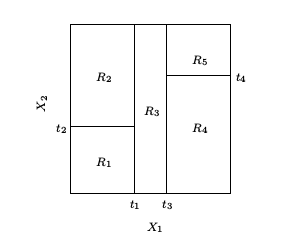
\includegraphics[width=0.9\textwidth]{figure/recursive_partitioning.png}
        \caption{Recursive partitioning of the feature space}
  \label{fig:rpart}
\end{figure}

Tree-based methods are supervised learners as they require the data to
either be labelled with a class or to have some outcome value.
\index{machine learning!supervised} The variable types in the feature
space (or vector space of the data)
\index{feature!space|seealso {vector space}} can be mixed. Because the
method cuts the vector space into a tiled surface (see figure
\ref{fig:rpart}), the features or data variables can be continuous or
discontinuous. The `simple models' that tree methods construct each
define one of the rectangular regions or partitions of the feature
space. In Figure \ref{fig:rpart}, the different regions or partitions
produced by a decision tree are labelled \(R1, R2\) etc.

\begin{table}[ht]
\centering
\begingroup\tiny
\begin{tabular}{lrr}
  \hline
Title & Year & Citations \\ 
  \hline
The Achievement Motive And Economic Behavior & 1964 &  20 \\ 
  Simplification Of Economic Models & 1966 &   9 \\ 
  Data Dredging Procedures In Survey Analysis & 1966 &  65 \\ 
  Advertising Performance As A Function Of Print Ad Characteristics & 1967 &  32 \\ 
  World Affairs Information And Mass Media Exposure & 1967 &  27 \\ 
  Juvenile Probation System Simulation For Research And Decision Making & 1968 &  16 \\ 
  Presidential Elections   Explanation Of Voting Defection & 1969 &  12 \\ 
  An Interactive Technique For Analysis Of Multivariate Data & 1969 &   9 \\ 
  Finding Variables That Work & 1969 &  22 \\ 
  Brand Trial After A Credibility Change & 1970 &   7 \\ 
   \hline
\end{tabular}
\endgroup
\caption{References to Morgan and Sonquist's Automatic Interaction Detector} 
\label{table:aid_citation}
\end{table}

\index{machine learner!decision tree!history of|(} Work on
classification and regression techniques using decision trees goes back
to the early 1960s when social scientists James Morgan and John Sonquist
at the University of Michigan's Institute for Social Research were
attempting to analyse increasingly large social survey datasets
\autocite{Morgan_1963}. As Dan Steinberg describes in his brief history
of decision trees \autocite[180]{Steinberg_2009}, the `automatic
interaction detector' (\texttt{AID}) as it was known, sought to automate
the practice of data analysts looking for interactions between different
variables. The variety and sheer optimism of subsequent applications of
these prototype decision tree techniques is striking. In the 1960s and
1970s, papers that drew on the AID paper or use AID techniques can be
found, as table \ref{table:aid_citation} shows, in education, politics,
economics, population control, advertising, mass media and family
planning. \index{machine learner!decision tree!history of}
\index{machine learner!automatic interaction detector}

\begin{figure}
  \centering
      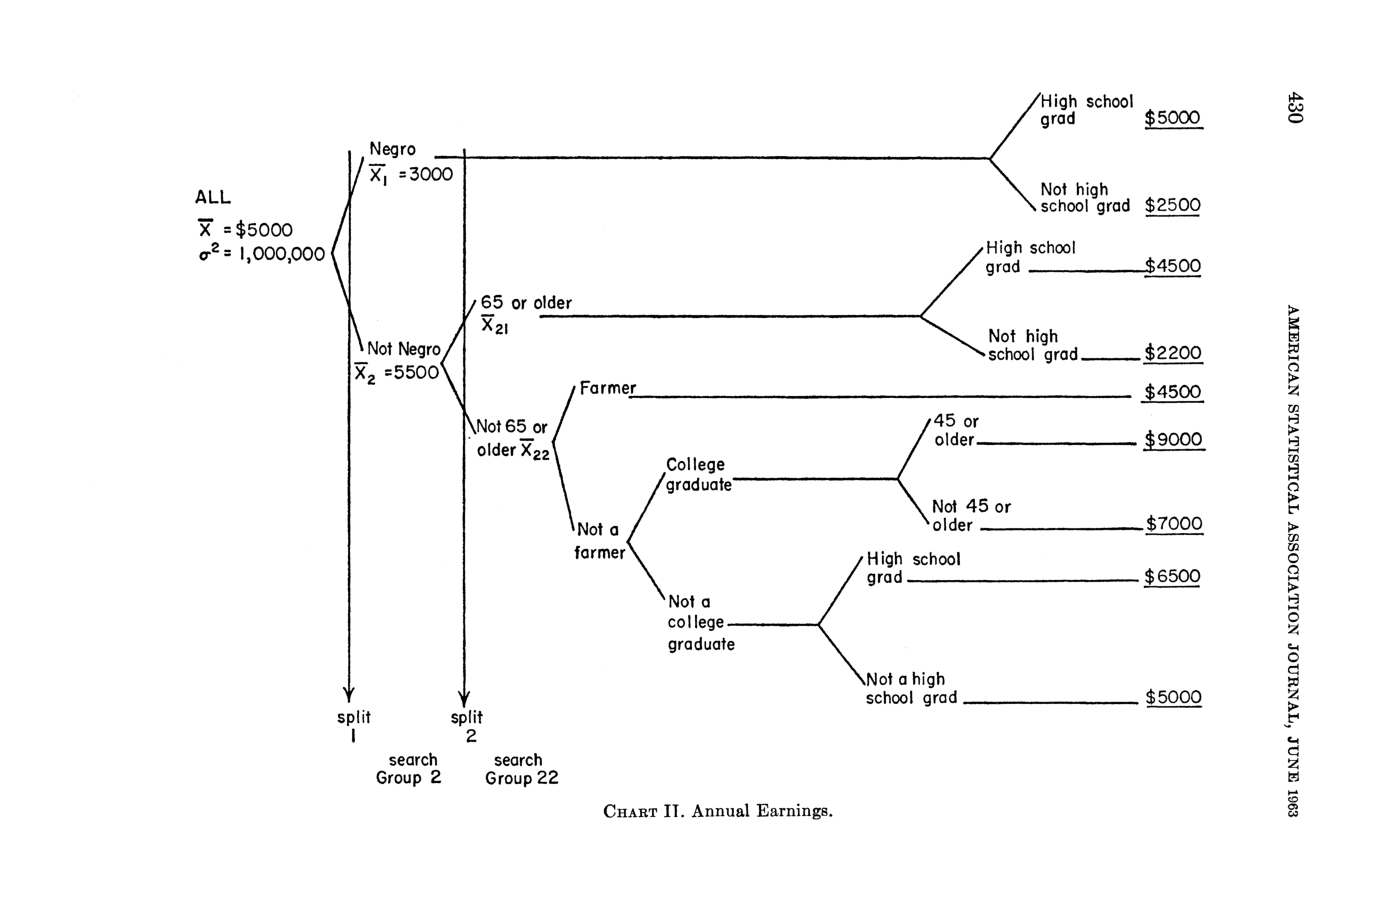
\includegraphics[width=0.9\textwidth]{figure/morgan_sonquist_p430.pdf}
        \caption[\texttt{AID classifier}]{AID classifies annual earnings (Morgan \& Sonquist, 1963, 430)}
  \label{fig:aid_tree}
\end{figure}

A decade after the initial work, \texttt{AID} was the object of
trenchant criticism by statisticians and others, not for the
classifications it used (see Figure \ref{fig:aid_tree}), but for its
`pure' empiricism. Writing in the 1970s, statisticians in the
behavioural sciences such as Hillel Einhorn at the University of Chicago
castigated the use of such techniques. The criticisms stemmed from a
general distrust of `purely empirical methods', and scepticism focused
on their positivity:

\begin{quote}
The purely empirical approach is particularly dangerous in an age when
computers and packaged programs are readily available, since there is
temptation to substitute immediate empirical analysis for more analytic
thought and theory building. It is also probably too much to hope that a
majority of researchers will take the time to find out how and why a
particular program works. The chief interest will continue to be in the
output-the results-with as little delay as possible
\autocite[368]{Einhorn_1972} \index{Hillel, Einhorn}
\end{quote}

Einhorn discusses AID alongside other techniques such as factor analysis
and multi-dimensional scaling (both still widely used) before concluding
`it should be clear that proceeding without a theory and with powerful
data analytic techniques can lead to large numbers of Type I errors'
\autocite[378]{Einhorn_1972}. His statistical objections to AID are
particularly focused on the problematic power of the technique: `it may
make sense out of ``noise''\,' (369). Consequently, researchers easily
misuse the technique: they `overfit' the data, and do not pay enough
attention to issues of validation (369-370). Similarly the British
marketing researcher Peter Doyle, criticising the use of AID in
assessing store performance and site selection by operations
researchers, complained that searching for patterns in data using data
sets was bound to lead to spurious results and the decision trees,
although intuitively appealing (that is, they could be easily
interpreted), were afflicted with arbitrariness: `a second variable may
be almost as discriminating as the one chosen, but if the program is
made to split on this, quite a different tree occurs'
\autocite[465-466]{Doyle_1973}.\footnote{These objections and
  resistances to early decision trees echo today in discussions around
  pattern recognition, knowledge discovery and data-mining in science
  and commerce. The problem of what computers do to the analysis of
  empirical data is long-standing.}
\index{operations research!use of decision trees}
\index{error!overfitting} Most of these criticisms can be seen as
expressing conventional statistical caution in response to threats to
validity, but they also address the core issues of pattern and
difference: did the trees render differences arbitrarily?
\index{machine learner!decision tree!history of|)}

\section{1984: Differences in recursive
partitioning}\label{differences-in-recursive-partitioning}

As Einhorn expected, it was too much to hope that all researchers would
take time to investigate how a particular program works. Some
researchers however did take time in the following decade to investigate
how decision trees work. Writing around 2000, Hastie, Tibshirani and
Friedman, who could hardly by accused of not understanding decision
trees, happily recommend decision trees as the best `off-the-shelf'
classifier: `of all the well-known learning methods, decision trees
comes closest to meeting the requirements for serving as an
off-the-shelf procedure for data-mining' \autocite[352]{Hastie_2009}. We
might wonder here, however, whether they damn with faint praise, since
`off-the-shelf' suggests pre-packaged, and commodified, and the term
`data-mining' itself is not without negative connotations. As for its
commercial realities, in 2013, Salford Systems, the purveyors of the
leading contemporary commercial decision tree software, \texttt{CART},
could claim:

\begin{quote}
CART is the ultimate classification tree that has revolutionized the
entire field of advanced analytics and inaugurated the current era of
data mining. CART, which is continually being improved, is one of the
most important tools in modern data mining. Others have tried to copy
CART but no one has succeeded as evidenced by unmatched accuracy,
performance, feature set, built-in automation and ease of use.
\href{http://www.salford-systems.com/products/cart}{Salford Systems}
\index{machine learner!CART}
\end{quote}

What happened between 1973 and 2013? Decision trees somehow stepped out
of the statistically murky waters of social science departments and
business schools in the early 1970s to inaugurate the `current era of
data mining' (which the scientific literature indicates starts in the
early 1990s). \index{data mining!in 1970} This was not only a commercial
innovation. As the earlier citation from U.S. National Institutes of
Health biostatisticians Malley, Malley and Pajevic indicates, decision
trees enjoy high regard even in biomedical research, a setting where
statistical rigour is highly valued for life and death reasons. The
happy situation of decision trees four decades on suggests some kind of
threshold was crossed in which the epistemological, statistical, or
algorithmic (`built-in automation') power of the technique altered
substantially. \index{machine learner!decision tree!in medicine}

The third author of \emph{Elements of Statistical Learning}, Jerome
Friedman, worked at the U.S. Department of Energy's Stanford Linear
Accelerator during the late 1970s. Friedman was instrumental in rescuing
decision trees from the ignominy of profligate ease of use and pure
empiricism they had endured since the late 1960s.
\index{Friedman, Jerome!work on decision tree} The reorganisation and
statistical retrofitting of the decision tree was not a single or
focused effort. During the 1980s, statisticians such as Friedman and Leo
Breiman renovated the decision tree as a statistical tool
\autocite{Breiman_1984}. At the same time, computer scientists such as
Ross Quinlan in Sydney were re-implementing decision trees guided by an
artificial intelligence-based formalisation as rule-based induction
technique \autocite{Quinlan_1986}.\footnote{Quinlan's papers and book on
  versions of the decision tree (\texttt{ID3} and \texttt{c4.5}) are
  both amongst the top ten the most highly cited references in the
  machine literature itself. Google Scholar reports over 20,00 citations
  of the Quinlan's book \emph{C4.5: Programs for Machine Learning}
  \autocite{Quinlan_1993} (although far fewer appear in Thomson Reuters
  Web of Science). Several years ago, \texttt{C4.5} was voted the top
  data mining algorithm \autocite{Wu_2008}. While I don't discuss
  Quinlan's work in much detail here, we should note as a computer
  scientist, Quinlan takes a much more rule-based approach to decision
  tree that Breiman and co-authors.
  \index{Quinlan, John Ross!induction tree}
  \index{machine learner!\texttt{C4.5}}} \index{Quinlan, John Ross!}
\index{artificial intelligence!rule-based induction} This uneasy
parallel effort between computer science and statistics still somewhat
strains relations in machine learning today. Statisticians and computer
scientists do and use the same techniques, but often with the computer
scientists focusing on optimisation and algorithmic scale and the
statisticians inventing novel statistical formalizations and
abstractions. The fateful embrace of statistics and computer science,
the disciplinary binary that vectorizes machine learning, has been
generative in the retrieval of the decision tree.
\index{statistics!relation to computer science}

An initial symptom of the transformation of the technique appears in a
name change. The term `decision tree,' although still widely used in the
research literature and machine learner parlance was supplanted by
`classification and regression tree' during the late 1970s and 1980s.
The terms `classification and regression tree' is sometimes contracted
to `CART,' and that term strictly speaking refers to a computer program
described in \autocite{Breiman_1984} as well as the title of that
highly-cited monograph, \emph{Classification and Regression Trees}.
\index{machine learner!CART} \index{Breiman, Leo!CART monograph} As we
have seen in previous chapters, classification and regression
(predictive modelling using estimates of relations between variables)
\index{regression|see {machine learner!linear regression}} stage the two
main sides of machine learning practice. Their concatenation with `tree'
attests to a renovation of existing machine learning approaches behind a
single facade.

The implementation of machine learning techniques in \texttt{R}
accentuates the statistical side of decision tree practice, but that has
certain forensic virtues not offered by commercial or closed-source
software often produced by computer scientists. The name of one
long-standing and widely-used \texttt{R} package itself attests to
something: \texttt{rpart} is a contraction of `recursive partitioning'
and this term generally describes how the decision tree algorithm works
to partition the vector space into the form shown in Figure
\ref{fig:rpart} \autocite{Therneau_2015}.
\index{R!packages!\texttt{rpart}} `CART,' on the other hand, is a
registered trademark of Salford Systems, the software company mentioned
above, who sell the leading commercial implementation of classification
and regression trees. Hence, the \texttt{R} package \texttt{rpart}
cannot call itself the more obvious name \texttt{cart,} and instead
invokes the underlying algorithmic process: recursive
partitioning.\footnote{Other \texttt{R} packages such as \texttt{party}
  \autocite{Hothorn_2006} and \texttt{tree} \autocite{Ripley_2014} also
  use recursive partitioning, but with various tweaks and optimisations
  that I leave aside here. \index{R!packages!\texttt{party}}
  \index{R!packages!\texttt{party}}}
\index{algorithm!recursive partitioning} \index{programming languages!R}

\begin{lstlisting}[language=R,caption={Decision tree for \texttt{iris} dataset}, label={rpart_iris}]
    data(iris)
    library(rpart)
    iris_tree =rpart(Species ~ ., iris)
\end{lstlisting}

R.A. Fisher's \texttt{iris} dataset, which contains 150 measurements
made in the 1930s of petal and sepal lengths of \emph{iris virginica,
iris setosa} and \emph{iris versicolor} is a standard instructional
example for decision trees \autocite{Fisher_1938}.\footnote{\texttt{iris}
  is a very small dataset, a pre-computational miniature.
  \index{dataset!iris} That diminutive character makes it
  diagrammatically mobile. It supports a rhizomatic ecosystem of
  examples scattered across the machine learning literature. The usual
  framing of the classification problem is how to decide whether a given
  iris blossom is of the species \emph{virginica}, \emph{setosa} or
  \_versicolor. These irises don't grow in forests -- they are more
  often found in riverbanks and meadows -- but they do offer a variety
  of illustrations of how machine learning classifiers are brought to
  bear on classification problems. Here the classification problem is
  taxonomic - the \emph{iris} genus has various sub-genera, and sections
  within the sub-genera.Setosa, \emph{virginica} and \emph{versicolor}
  all belong to the sub-genus \emph{Limniris}. This botanical context is
  routinely ignored in machine learning applications. In machine
  learning textbooks and tutorials, \texttt{iris} typically would be
  used to demonstrate how cleanly a classifier can separate the
  different kinds of irises. \index{dataset!\texttt{iris}}}
\index{dataset!\texttt{iris}} The code shown here loads the
\texttt{iris} data (the dataset is routinely installed with many data
analysis tools), loads the \texttt{rpart} decision tree library, and
builds a decision to classify the irises by species. What has happened
to the iris data in this decision tree? The \texttt{R} code that invokes
the recursive partitioning algorithm is so brief
\texttt{iris\_tree\ =rpart(Species\ \textasciitilde{}\ .,\ iris)} that
we can't tell much about how the data has been `recursively
partitioned.' We know that the \emph{iris} has 150 rows, and that there
are equal numbers of the three iris varieties.

Code brevity indicates a great deal of formalization of practice has
accrued around decision trees. \index{code!brevity of!} Some of this
formalization was described in the landmark \emph{Classification and
Regression Trees} monograph \autocite{Breiman_1984}. Classification in
decision trees operates by splitting each of the dimensions of vector
space into two parts (as we saw in figure \ref{fig:rpart}). These splits
institute branches along which differences are hierarchically ordered in
a tree structure. The recursive splitting algorithm draws a diagram of
hierarchical differences. The problem here is that many splits are
possible. What is a good split or ordering of differences?
\index{differences!ordering of}

\begin{quote}
The first problem in tree construction is how to use \(\mathcal{L}\) to
determine the binary splits of \(\mathcal{X}\) into smaller pieces. The
fundamental idea is to select each split of a subset so that the data in
each of the descendant subsets are ``purer'' than the data in the parent
subset \autocite[23]{Breiman_1984}.
\end{quote}

Tree construction hinges on the notion of purity or more precisely `node
impurity', a function that measures to what extent data labelled as
belonging to different classes are mixed together at a given branch or
node in a decision tree: `that is, the node impurity is largest when all
classes are equally mixed together in it, and smallest when the node
contains only one class' \autocite[24]{Breiman_1984}. As Malley and
co-authors note, `the collection of purity measures is still a subject
of research' \autocite[123]{Malley_2011}, but Breiman, Friedman, Olshen
and Stone promoted a particular form of impurity measure for
classification trees known as `Gini index of diversity'
\autocite[38]{Breiman_1984}. \index{difference!Gini index of diversity}
Like the planar decision surface used in classifiers such as the
perceptron or linear regression model, recursive partitioning combined
with measures of node impurity transforms data by cuts or
divides.\index{learning!as dividing} Whereas in linear model-based
machine learners, the intuition motivating the function-finding or
learning was `find the line that best expresses the distribution of the
data, \index{machine learner!logistic regression!gradient descent} here
the intuition is more like: 'find the cuts that minimize mixing'. Good
splits decrease the level of impurity in the tree. In a tree with
maximum purity, each terminal node -- the nodes at the base of the tree
-- would contain a single class.

\begin{figure}
  \centering
      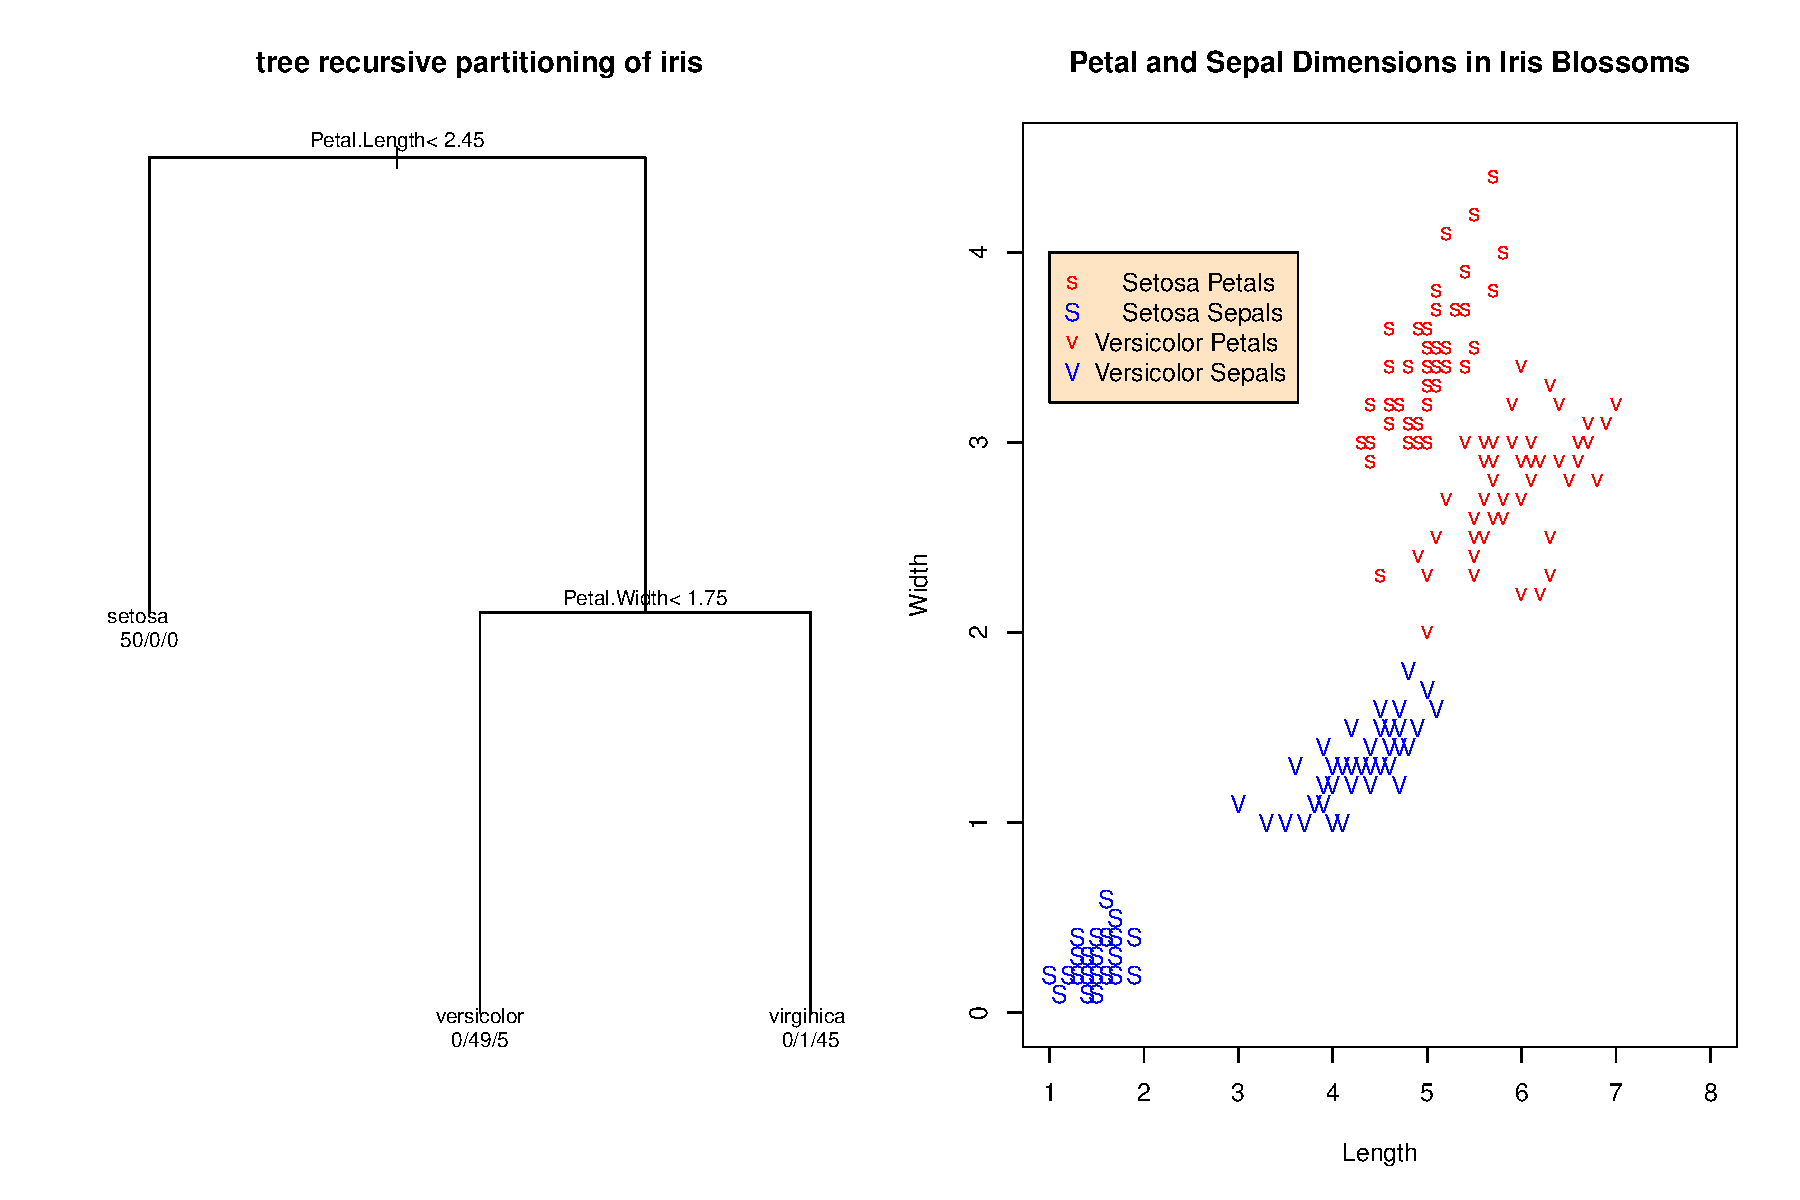
\includegraphics[width=0.9\textwidth]{figure/iris_tree_plot-1.pdf}
        \caption{Decision tree on \texttt{iris} dataset}
  \label{fig:iris_tree_plot}
\end{figure}

In Figure \ref{fig:iris_tree_plot}, the plot on the left shows the
decision tree and the plot on the right shows just \emph{setosa} and
\emph{versicolor} plotted by petal and sepal widths and lengths.
Decision trees are read from the top down, left to right. The top level
of this tree can be read, for instance, as saying, if the length of
petal is less 2.45, then the iris is \emph{setosa}. \index{dataset!iris}
As the plot on the right shows, most of the measurements are well
clustered. Only the \emph{setosa} petal lengths and widths seem to vary
widely. All the other measurements are tightly bunched. A decision tree
has little trouble ordering differences between species of iris.

Like logistic regression models, neural networks, support vector
machines or any other machine learning technique, decision trees order
differences in terms of specific qualities and logics. Recursive
partitioning split and sub-divide the vector space to capture every
minor difference between cases, and thereby achieve a ever-closer fit to
the individual or sub-individual variations.
\index{algorithm!recursive partitioning} Although the partitioning or
splitting rules have strong statistical justifications, they do not at
all eliminate the problem of instability or variance in trees.
\index{error!variance} For instance, they easily end up `overfitting'
the data. Overfitting is a problem for all machine learning techniques.
Algorithms sometimes find it hard to know when to stop identifying
differences. During construction of a decision tree, recursive
partitioning splits features in the data into smaller and smaller
groups. `The goodness of the split', wrote Breiman and co-authors, `is
defined to be the decrease in impurity' \autocite[25]{Breiman_1984}.
Under this definition of goodness, the terminal nodes or leaves of the
tree can end up containing a single case, or a single class of cases.
\index{differences!defined as purity}

The decision tree targets the differences of the individual case to such
a degree that it could end up seeing categorical differences everywhere.
Operating to maximise the purity of the partitions it creates, it leans
too heavily on data it has been trained on to see relevant similarities
when fresh data appears. Trees that branch too much are sensitive to
differences and generalize poorly (that is, they suffer from
generalization error \textbackslash{}index\{error!generalization\}).
Such a model will almost always \emph{overfit}, since slight variations
in the values of variables in a fresh case are likely to yield widely
differing predictions. In the terminology of machine learning, such a
decision tree may have low bias but high variance.
\index{error!overfitting}\index{model!overfitting}
\index{error!bias-variance}

\section{Limiting differences}\label{limiting-differences}

Given this problem of unstable difference, much of the development of
decision tree did not revolve around how to construct them, but how to
limit their growth so as to manage tensions between pure but unstable
differences and impure but stable classification. As \emph{Elements of
Statistical Learning} puts the problem in its account of classification
and regression trees:

\begin{quote}
How large should we grow the tree? Clearly a very large tree might
overfit the data, while a small tree might not capture the important
structure. Tree size is a tuning parameter governing the model's
complexity, and the optimal tree size should be adaptively chosen from
the data. One approach would be to split tree nodes only if the decrease
in sum-of-squares due to the split exceeds some threshold. This strategy
is too short-sighted, however, since a seemingly worthless split might
lead to a very good split below it. The preferred strategy is to grow a
large tree \(T_0\), stopping the splitting process only when some
minimum node size (say 5) is reached. Then this large tree is pruned
using cost-complexity pruning \autocite[307-308]{Hastie_2009}.
\end{quote}

Growing a maximum decision tree, and then cutting back its branches
using a cost-function \index{function!cost!complexity} optimises the
decision tree as a machine learner. \index{optimisation!decision tree}
\index{machine learner!decision tree!pruning} `Cost complexity pruning'
extends the optimisation we have already discussed in relation to linear
regression and logistic regression models (in chapter
\ref{ch:function}). As in these techniques, the definition of a cost
function controlling the `complexity' of a tree -- how many branches and
leaves/nodes it contains, combined with measures of how well it
classifies or predicts -- iteratively observes and tests different
versions of tree against each other. `We define the cost complexity
criterion,' write Hastie and co-authors, as:

\begin {equation}
\label {eq:tree_model}
C_\alpha(T) = \sum_{m=1}^{|T|}N_mQ_m(T) + \alpha|T|
\end {equation}

The idea is `to find, for each \(\alpha\), the subtree
\(T_\alpha \subseteq T_0\) to minimize \(C_\alpha(T)\)'
\autocite[308]{Hastie_2009}. For present purposes, we need only
recognise that the cost complexity function re-configures a large
decision tree (\(T_0\) in equation \ref{eq:tree_model}) by cutting or
pruning it back through optimisation that balances between the
complexity of the tree and its stability. Tree construction is as an
optimisation problem, in which the variation of a parameter (\(\alpha\))
allows minimization of a derived value (the cost \(C_\alpha\)).
\index{function!cost}

While the graphic form of the decision tree was, by virtue of the
long-standing diagrammatic practice of tree-drawing, easy to interpret,
observation of decision trees had no way of gauging the instability or
variability of any given tree. \index{diagram!decision tree as} Hastie
and co-authors write: 'one major problem with trees is their high
variance. Often a small change in the data can result in a very
different series of splits, making interpretation somewhat precarious.
The major reason for this instability is the hierarchical nature of the
process: the effect of an error in the top split is propagated down to
all of the splits below it \autocite[312]{Hastie_2009}. The very
diagrammatic form that allows decision trees to be observed and
interpreted is also the source of their instability. Regardless of this
instability, the diagrammatic composition of the tree through splitting
and pruning negotiates between two different ways of doing difference.

The shift from \texttt{AID} to \texttt{CART} enunciates a change in how
patterns of difference become visible. The decision tree algorithm
superimposes recursive partitioning and cost-complexity pruning to
configure a mode of enunciation of differences. It creates a new rules
of differentiation of individuals, facts, things and
relations.{[}\^{}5.101{]} Differences in a decision tree -- the
combination of purity and density that comes from recursive partitioning
and cost-complexity pruning -- re-configure what counts as pattern.
\index{differences!differentiation of}

Decision trees have been heavily used in credit risk assessment as well
as many biomedical models. Does their popularity stem from the
legibility of the statements they produce, even if those patterns prove
unstable? Or is the success of the decision tree perhaps better
understood as a change in the differentiation of patterns more
generally, their mode of enunciation, in which case, decision trees
would only be one instance among many? \index{enunciative modality} If
we understand machine learners as generating populations of statements,
the transformation and re-modelling of the decision tree as
classification and regression trees suggests a subtle, non-localizable
discontinuity. The later development of the decision tree and its
subsequent transmogrification into random forests
\autocite{Breiman_2001}, \index{machine learner!random forest} that grow
a myriad of small decision trees disperses kaleidoscopic fragments of
classificatory order with only partial or provisional stabilisation in
visible pattern. In such developments -- and we could also consider here
techniques, models and methods of `boosting,' `bagging,' or the
`ensemble learning' that conducts `supervised search in a
high-dimensional space of weak learners' \autocite[603]{Hastie_2009},
pattern has an operational rather than visible mode of togetherness.
\index{pattern!operational}

\section{The successful dispersion of the support vector
machine}\label{the-successful-dispersion-of-the-support-vector-machine}

In growing and pruning decision trees, and even more markedly in support
vector machine, patterns play out in dispersion and discontinuity rather
than in regular geometry. \index{pattern!in dispersion} While machine
learners order differences, that ordering becomes increasingly difficult
to see as it is dispersed. Take the case of the support vector machine.
The second most highly cited reference in the last few decades of
machine learning literature is a paper from 1995 by Corinna Cortes and
Vladimir Vapnik of AT \& T Bell Labs in New Jersey, USA entitled
`Support Vector Networks' \autocite{Cortes_1995}. Few women's names
appear prominently in the machine learning literature.
\index{sites!Stanford University}
\index{sites!AT \& T Bell Laboratories} \index{sites!Google Research}
The computing science and statistics departments at Stanford and
Berkeley, the laboratories at Los Alamos and AT\&T Bell between the
1960s and the 1980s were, it seems, not overly popular or populated with
women scientists and engineers. Some prominent machine learning
researchers at the time of writing are women (I return to this in
chapter \ref{ch:subjects}), but Cortes is perhaps pre-eminent both as
head of Google Research in New York (2014) and as recipient with Vapnik
of an Association for Computing Machine award in 2008 for work on the
support vector machine algorithm.\footnote{The support vector machine is
  distinctive in its transformations of data, and this owes something to
  history, politics and geography. Vapnik trained and worked of decades
  in the former USSR as a mathematician and statistician. His writings
  on the problems of pattern recognition contrast greatly with other
  engineers, statisticians and computer scientists in their robustly
  theoretical formalism. A highly cited 1971 publication with Alexey
  Chervonenkis `On the uniform convergence of relative frequencies of
  events to their probabilities' (published in Russian in 1968 )
  \autocite{Vapnik_1971} sets the formal tone of this work. In ensuing
  publications in Russian and then in English after Vapnik moved from
  Moscow to AT\&T's New Jersey Bell Labs in 1990, Vapnik's work remains
  quite formally mathematical. Although it pertains to `learning
  machines,' machine here are understood mathematically simply as `the
  implementation of a set of functions' \autocite[17]{Vapnik_1999}.
  \index{Vapnik, Vladimir} The way that Vapnik develops a theory of
  learning owes little visible debt to actual attempts to work with data
  or experience in doing statistics in any particular domain. This
  contrasts greatly for instance with the work of statisticians like
  Breiman or Friedman or even computer scientists like Quinlan or Le Cun
  whose work lies much closer to fields of application. Vapnik's work,
  like that of the Russian mathematician Andrey Kolmogorov he draws on,
  differs from many other contributions to machine learning partly by
  virtue of this formality and its efforts to derive insight into
  machine learning by theorising learning. The \emph{Vapnik-Chervonenkis
  dimension}( VC dimension), a very widely used way of defining the
  capacity of a particular machine learning technique to recognise
  patterns in data dates from his work in the 1960s and underpins a
  general theory of `learning.' Vapnik writes in 1995,
  \index{pattern!Vapnik-Chervonenkis dimension of}

  \begin{quote}
  The VC dimension of the set of functions (rather than the number of
  parameters) is responsible for the generalization ability of learning
  machines. This opens remarkable opportunities to overcome the ``curse
  of dimensionality \autocite[83]{Vapnik_1999}.
  \end{quote}

  As we will see in this chapter, Vapnik's attempts to overcome
  dimensionality also re-shape what counts as pattern.
  \index{Vapnik, Vladimir!biography}} \index{Cortes, Corinna}
\index{Vapnik, Vladimir}
\index{support vector machine|see{machine learner!support vector machine}}

\begin{table}[ht]
\centering
\begingroup\tiny
\begin{tabular}{p{0.7\textwidth}p{0.1\textwidth}p{0.15\textwidth}}
  \hline
Title & Year & Citations \\ 
  \hline
A tutorial on Support Vector Machines for pattern recognition & 1998 & 3510 \\ 
  Support vector machine classification and validation of cancer tissue samples using microarray expression data & 2000 & 869 \\ 
  Choosing multiple parameters for support vector machines & 2002 & 681 \\ 
  Classification of hyperspectral remote sensing images with support vector machines & 2004 & 428 \\ 
  Comparing support vector machines with Gaussian kernels to radial basis function classifiers & 1997 & 405 \\ 
  Support Vector Machines for 3D object recognition & 1998 & 396 \\ 
  An assessment of support vector machines for land cover classification & 2002 & 295 \\ 
  Drug design by machine learning: support vector machines for pharmaceutical data analysis & 2001 & 273 \\ 
  A novel method of protein secondary structure prediction with high segment overlap measure: Support vector machine approach & 2001 & 266 \\ 
  LIBSVM: A Library for Support Vector Machines & 2011 & 246 \\ 
  The entire regularization path for the support vector machine & 2004 & 223 \\ 
  A GA-based feature selection and parameters optimization for support vector machines & 2006 & 223 \\ 
  The support vector machine under test & 2003 & 219 \\ 
  Credit rating analysis with support vector machines and neural networks: a market comparative study & 2004 & 218 \\ 
   \hline
\end{tabular}
\endgroup
\caption{Most cited papers on support vector machines} 
\label{tab:svm_lit}
\end{table}

The rapid rise to popularity of the support vector machine can be seen
in the machine learning research literature, a very small slice of which
appears in Table \ref{tab:svm_lit}. A substantial fraction of the
overall research publication since the mid-1990s accumulates around this
single technique, and as usual ranges across credit analysis, land cover
prediction, protein structures, brain states and face recognition. The
support vector machine spans the normal biopolitical triangle of life,
labour and language. The influence of the technique can also be seen in
overlapping fields such as pattern recognition and data mining, where
\autocite{Cortes_1995} and similar papers rank near the top-cited
papers.\footnote{\emph{Elements of Statistical Learning} also devotes a
  chapter to support vector machines \autocite[Chapter 14]{Hastie_2009}}
This kind of growth betokens high levels of interest, identification and
investment on the part of the researchers, and presumably more widely.

\begin{figure}
  \centering
      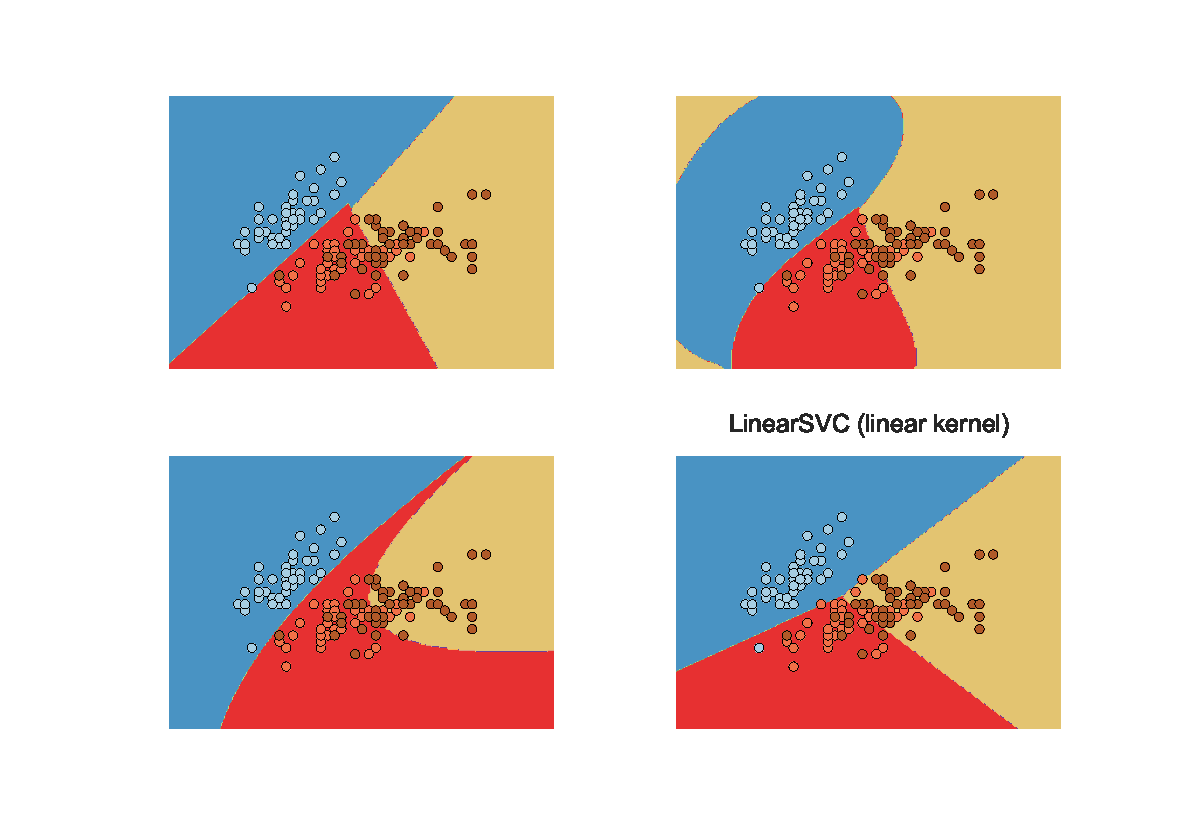
\includegraphics[width=1.0\textwidth]{figure/contour.pdf}
        \caption{Support vector machine on \texttt{iris} dataset}
  \label{fig:svm_iris}
\end{figure}

I suggested above that the classification tree (and then random forests)
illustrate an enunciative modality anchored in a tension between
recursively partitioned differences and classificatory stability.
\index{referential!dispersed} The support vector machine shown in Figure
\ref{fig:svm_iris} demonstrates a different change in what counts as
pattern. The decision boundaries in the sub-graphs have different
contours, contours that suggest a more mobile construction. While the
name `support vector machine' is somewhat forbiddingly technical
compared to more familiar terms such as `decision tree' or even `neural
network,' the underlying intuition of the technique is much older, and
can be found in the models developed by the British statistician R. A.
Fisher during the 1930s. Fisher developed the `first pattern recognition
algorithm' \autocite[273]{Cortes_1995}, the `linear discriminator
function' \autocite{Fisher_1936}, to deal with problems of
classification, and demonstrated its efficacy on the taxonomic problem
of discriminating or classifying the irises observed in W.E. Anderson's
irises in \texttt{iris} dataset (see above). \index{dataset!iris}
\index{function!linear discrimant}
\index{machine learner!linear discriminant analysis}

In his 1936 article in the \emph{Annual Review of Eugenics}, Fisher
comments on similar classification work carried out in craniometry and
other related settings: so-called `discriminant functions' had been
successfully used to distinguish populations. Fisher wrote: `when two or
more populations have been measured in several characters, \ldots{}
special interest attaches to certain linear functions of measurements by
which the populations are best discriminated'
\autocite[179]{Fisher_1936}. \index{Fisher, Ronald Ayre} The
discriminant functions divide the vector space into `a collection of
regions labeled according to classification'
\autocite[101]{Hastie_2009}. `Decision boundaries' (or sometimes
`decision surfaces' \index{classification!decision boundary} often
appear as straight lines that divide the vector space into regions of
constant classification. \index{function!discriminant} These
long-standing discriminant functions were reconstructed during the 1990s
in the form of the support vector machine, giving rise to new statements
about differences, statements that can be glimpsed in table
\ref{tab:svm_lit} in the range of things, facts and beings running
through the titles of the papers.

\section{Differences blur?}\label{differences-blur}

Decision boundaries change in two ways in support vector machines. They
blur and bend, again affecting what counts as pattern.
\index{pattern!dispersion of} The support vector machine addresses the
problem of how to model differences when differences are blurred. An
oft-repeated illustration of how the support vector machine transforms
data appears in Cortes and Vapnik's initial publication simply entitled
`Support Vector Networks' \autocite{Cortes_1995}. They demonstrate how
the support vector machine classifies handwritten digits drawn from a
dataset supplied by the US Postal Service \autocite{LeCun_2012}. Like
\texttt{iris}, the US Postal Service digits and a larger version from
the US National Institute of Standard (\texttt{mnist}) are standard
machine learning dataset. They have been frequently used to measure the
performance of competing learning algorithms.
\index{dataset!U.S. Postal digits|see{dataset!\texttt{mnist}}} In
contrast to \texttt{iris}, the \texttt{mnist} is high dimensional. Each
digit in the dataset is stored as a 16x16 pixel image. Image
classification typically treats each pixel as a feature or variable in
the input space. So each digit as represented by 16x16 pixels amounts to
a 256 dimensional input space.\index{data!image as} By comparison,
\texttt{iris} has five dimensions. Unsurprisingly, there are also many
more digits in the US Postal Service Database than in flowers in
\texttt{iris}. The \texttt{mnist} dataset has around 70,000. Aside from
this dimensional growth, the handwritten digits aptly convey the
blurring of differences. On the one hand, many people can easily
recognise slight variations in handwritten digits with few errors. This
is despite the many variations in handwriting that skew, morph and
distort the ideal graphic forms of numbers.\footnote{Neural network
  researchers have heavily used the MNIST dataset. I discuss some of
  that work in chapter \ref{ch:subjects}. The handwritten MNIST also
  appear in \emph{Elements of Statistical Learning} , where they are
  used to compare the generalization error (see previous chapter) of a
  \emph{k} nearest neighbours, convolutional neural network, and a
  `degree-9 polynomial' support vector machine
  \autocite[408]{Hastie_2009}. \index{dataset!\texttt{mnist}} What about
  the handwritten digits attracts so many machine learning techniques?
  The logistics of the US Postal Service aside (since the \texttt{mnist}
  datasets continue to be used by machine learners well after the
  problem of scrawl on letters has been sorted), the variations, the
  regularities, and the banal everydayness of these digits furnish a
  referential locus, whose existence as a facts, things or events in the
  world is less important than the relations of similarity and
  differences it poses. \index{referential} The field of digitals
  becomes a site of differentiation not only of digits -- the machine
  learners attempt to correctly classify the digits -- but of the
  authority of different machine learning techniques and approaches.
  They become ways of announcing and delimiting the authority, the
  knowledge claims or `truth' associated with the machine. The many uses
  of the\texttt{mnist} data documented by \autocite{LeCun_2012} suggests
  something of the ancestral probabilisaton
  \index{probabilisation!ancestral} of such datasets.}

\begin{figure}
  \centering
      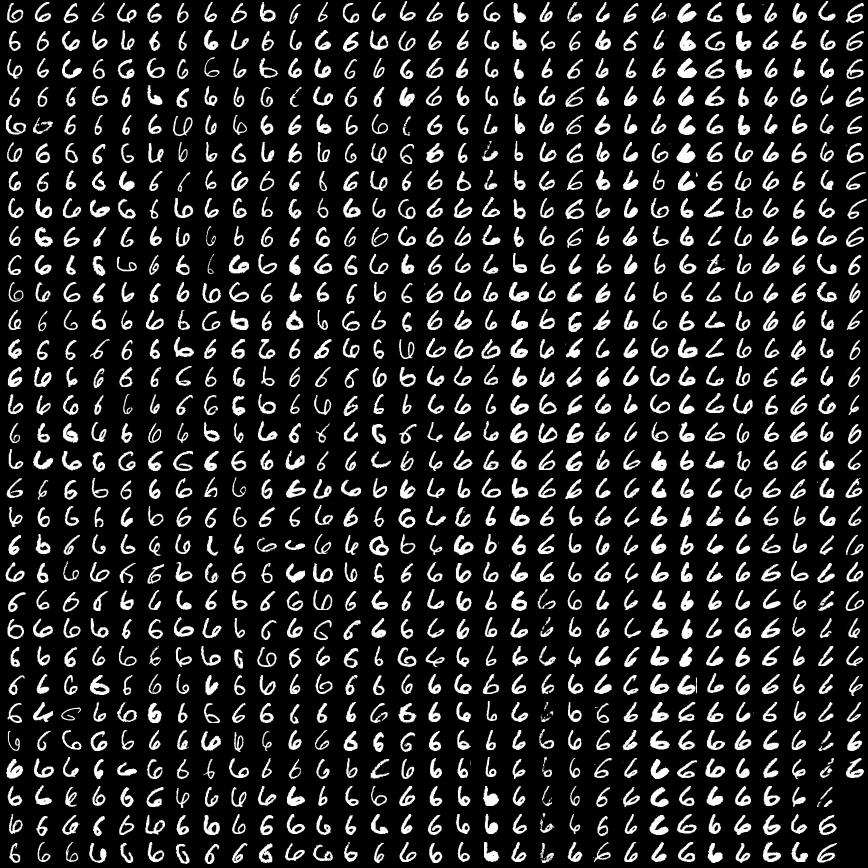
\includegraphics[width=0.9\textwidth]{figure/mnist_test6.jpg}
        \caption{MNIST Postal Digits}
  \label{fig:postal_digits}
\end{figure}

In their experiments with digit recognition (shown in figure
\ref{fig:postal_digits}, Cortes and Vapnik contrast the error rates of
decision trees (\texttt{CART} and \texttt{C4.5}), neural networks and
the support vector machine working at various level of dimensionality.
Support vector machines deal with blurred differences or continuous
variations by superimposing two operations: `soft margins' and
`kernelisation.' Nearly all expositions of the support vector machine
including \autocite{Cortes_1995} highlight the `soft margin' that runs
in parallel to the solid decision boundary. The support vector machine
develops Fisher's linear discriminant analysis since it searches for a
separating hyperplane in the data.
\index{hyperplane|see{decision surface}} While linear discriminant
analysis constructs a hyperplane by finding the most likely linear
boundary between classes based on all the data, the support vector
machine searches for a hyperplane resting only on those cases in the
data that lie near the boundary. It introduces the intuition that the
best hyperplane differentiating classes will run near to the cases --
the \emph{support vectors} -- that are most difficult to classify.
Hard-to-classify cases become the `support vectors'
\index{machine learner!support vector machine!support vectors in} whose
relative proximities tilt the decision surface in various directions. In
contra-distinction to the \(N=\forall{\boldsymbol{X}}\) proposition
(discussed in chapter \ref{ch:probability}), the machine learner
discards much of the data. In contrast to linear discriminant analysis,
as Ethem Alpayadin writes, `we do not care about correctly estimating
the densities {[}probability distributions of variables{]} inside class
regions; all we care about is the correct estimation of the
\emph{boundaries} between the class regions'
\autocite[210]{Alpaydin_2010}.
\index{Alpaydin, Ethem!on decision boundaries}
\index{machine learner!linear discriminant analysis}

\begin{figure}
  \centering
      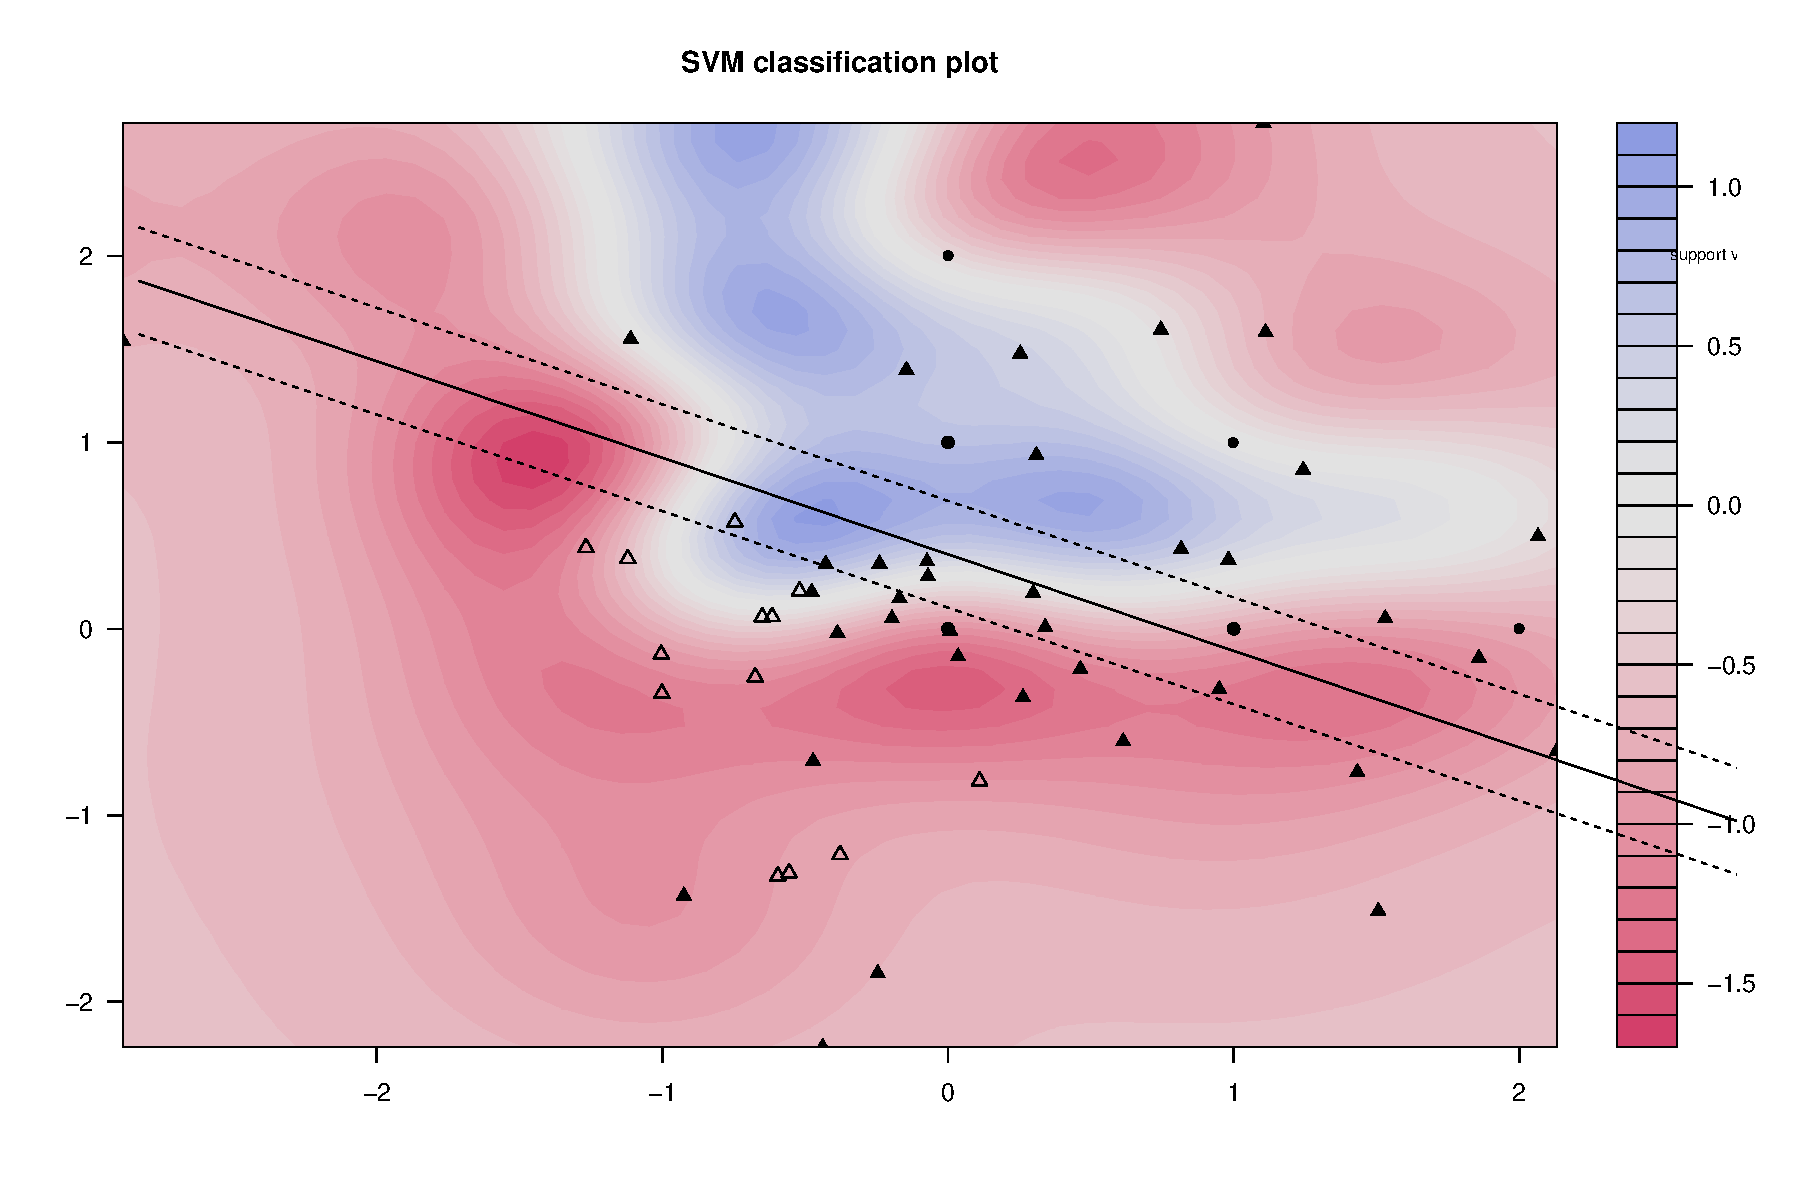
\includegraphics[width=0.9\textwidth]{figure/svm_margins-1.pdf}
    \caption[Margins in a support vector machine]{Margins in a support vector machine. The margins ignore most of the data and only focus on the hard-to-classify cases}
  \label{fig:svm_margins}
\end{figure}

Figure \ref{fig:svm_margins} has appeared in many slight variations in
the last two decades. Such figures diagram classes by different point
shapes, and the diagrammatic work of the classifier takes the shape of
diagonal lines, the solid line marking the decision surface or
hyperplane and the dotted lines marking the soft margins that separate
the two classes. In Figure \ref{fig:svm_margins}, the dotted lines
represent a margin on either side of a hyperplane (the solid line). The
support vector machine finds the hyperplane for which that margin or
perpendicular distance between the margins is greatest. Of all the
slightly different planes that might run between the two classes shown
in that figure, the maximum separating hyperplane lies at the greatest
distance from all the points of the different classes. The support
vector classifier modifies the idea of the optimal separating hyperplane
by accommodating inseparable or overlapping classes. This is something
that other machine learners (for instance, the perceptron) cannot do.
\index{differences!overlapping}

While the geometrical intuition here is that some data points (cases or
observations) will lie on the opposite side of the decision surface to
where they should be, the distance they lie on the wrong side of the
separating hyperplane will be as small as possible. How are the lines
showing in Figure \ref{fig:svm_margins} calculated? Locating the optimal
separating hyperplane and a limited number of permitted
mis-classifications presents a complicated optimisation problem. As
\emph{Elements of Statistical Learning}, following Cortes and Vapnik's
formulations, formalizes it, the problem can be stated in terms of
minimization:

\begin {equation}
\label {eq:lagrange_primal}
L_P = \frac{1}{2}\parallel\beta\parallel^2 + C\sum_{i=1}^{N}\xi_i - \sum \alpha[y_{i}(x_i^T\beta + \beta_0) - (1-\xi_i)]- \sum_{i=1}^{N}\mu_i\xi_i
\end {equation}

\autocite[420]{Hastie_2009}

In equation \ref{eq:lagrange_primal}, the optimisation problem is to
minimize \(L_P\), the Lagrange primal function with respect to
\(\beta, \beta_0\) and \(\xi_i\) \autocite[420]{Hastie_2009}.
\index{optimisation!Langrange Primal function} In this complicated
optimisation problem (one that is difficult to understand without
extensive mathematical background), familiar elements include the
parameters \(\beta\) in the linear form of \(x_i^T\beta + \beta_0\),
which is the equation defining the hyperplane, as well as triple
operations of addition (\(\sum\)) of all the values \(\xi_i\), which
calculate the distance that each case is on the wrong side of the
margin. Correctly classified cases will, therefore, have \(x_i =0\).

As always with mathematical functions, their diagrammatic relations, and
the way in which they contain both the generalizing regularities
(algebraic icons and indexes, the linear equation, the repeated
summation of all values, the shaping parameters) and forms of variation
(the presence of the misclassification measures \(\xi_i\)) should focus
our attention. What if elements that lie on the wrong side of the
hyperplane were allowed? If that were possible, the support vector
machine could deal with in-separable or overlapping classes, and hence
with blurred patterns of difference. Given that support vector machine
permits instances that lie on the wrong side of the separating
hyperplane, irregular differences no longer function as errors (as they
would appear in most linear classifiers such as linear discriminant
analysis and logistic regression), but as elements in a `soft margin'
designed to accommodate inseparability and indistinctness. Equations
such as equation \ref{eq:lagrange_primal} connect the diagrammatic
intuition of a separating hyperplane with a set of steering movements
controlled by parameters such as \(C\), which effectively controls the
size of the margin, and \(\alpha\), which effectively bounds the
proportion by which a predicted instance can be on the wrong side of the
margins that define the hyperplane. In other words, as we have seen
previously in cost-function optimisation (see chapter
\ref{ch:function}), the learning in the machine consists in finding a
way of transforming data into differences according to constraints.
\index{diagram!forms of movement}

\section{Bending the decision
boundary}\label{bending-the-decision-boundary}

The support vector machine reinstates a linear decision boundary as the
enunciative mode of
difference.\index{enunciative modality!of differences} Yet it transforms
that boundary. In the abstract of their 1995 paper, Cortes and Vapnik
briefly describe the how the support vector machine revises the linear
decision surface:

\begin{quote}
The support-vector network is a new learning machine for two-group
classification problems. The machine conceptually implements the
following idea: input vectors are non-linearly mapped to a very
high-dimension feature space. In this feature space a linear decision
surface is constructed \autocite[273]{Cortes_1995}
\index{machine learner!support vector machine!non-linear mapping in}
\end{quote}

Another example of vector space transformation (discussed in chapter
\ref{ch:vector}),\index{vector space!transformation of} this `very
high-dimension feature space' is explicitly made to support `a linear
decision surface,' just as Fisher's linear discriminant analysis had.
But this linear decision surface is now located amidst a non-linear
mapping of the data.\footnote{As we have seen on several occasions, the
  vector space invites a certain form of classification based on the
  search for the best line, the line of best fit, or the most
  discriminating line, the line that best divides things from each
  other. Linear regression is not called `linear' for no reason. And
  Fisher's `discriminant functions' were later called `linear
  discriminant analysis' for the same reason: they divide the vector
  space into different regions (`decision regions') separated by `linear
  decision boundaries' \autocite[53]{Alpaydin_2010}. Almost all machine
  learners are aware of and try to address the idealism or abstraction
  of the line or plane. \index{abstraction!of line and plane}} Cortes
and Vapnik's support vector machine constructs a new domain - `a very
high dimension feature space' -- where inseparable differences start to
disentangle themselves. The constructed dimensions do not index new
sources or kinds of data. Instead, the support vector machine transforms
the vector space into a much higher dimension.

As Vapnik writes in the preface to the second edition of \emph{The
Nature of Statistical Learning Theory} \autocite[vii]{Vapnik_1999}, `in
contrast to classical methods of statistics where in order to control
performance one decreases the dimensionality of a feature space, the SVM
dramatically increases dimensionality' (vii).
\index{Vapnik, Vladimir!dimensional increase} From the standpoint of
pattern recognition, this often vastly augmented vector space should
make it harder to locate patterns. A linear or planar decision surface
in high dimensional space maps onto a curving even labyrinthine decision
boundary when projected back onto the original vector space (see the
curving decision boundaries in figure \ref{fig:svm_iris}). In certain
cases, machine learners multiply dimensions in data in the name of
differentiation, classification, and prediction. Many of the techniques
that have accumulated or been gathered into machine learning flatten
variations and differences into lines and planes, but not always by
reducing them. In fact, random forests, neural networks and support
vector machines exemplify a counter-movement that maximises variety in
the name of differentiation.\footnote{Despite the in-principle
  commitment to any form of function, machine learning strongly prefers
  forms that can either be visualised on a plane (using the visual
  grammar of lines, dots, axes, labels, colours, shapes, etc.), or can
  be computed in form of matrix or vectorised calculations focused on
  planes. \index{vectorisation} Many of the techniques that grapple with
  complicated datasets seek to reduce their dimensionality so that
  lines, planes and regular curves can be applied to them:
  multi-dimensional scaling (MDS), factor analysis, principal component
  analysis (PCA), or self-organising maps (SOM) are just a few examples
  of this. \index{function!linear}
  \index{machine learner!principal component analysis}
  \index{machine learner!multidimensional scaling}
  \index{machine learner!self-organizing maps}} Research in machine
learning, whether it has been primarily statistical, mathematical or
computational, countenances and addresses problems of non-linear
classification through \emph{dimensional expansion}.
\index{vector space!dimensionality}

The powerful augmentation characteristic of the support vector machine
works through diagrammatic substitution.
\index{diagrammatic!substitution} Consider the expression shown below in
equation \ref{eq:kernel_model}:

\begin {equation} 
L_D = \sum_{i=1}^{N} \alpha_i - \frac{1}{2}\sum_{i=1}^{N}\sum_{i'=1}^{N}\alpha_i \alpha_{i'} y_{i} y_{i'}\langle h(x_i), h(x_{i'})\rangle
\label {eq:kernel_model}
\end {equation}

\autocite[423]{Hastie_2009}

In equation \ref{eq:kernel_model}, a re-mapping of equation
\ref{eq:langrange_primal} occurs particularly through the substitution
of a product \(\langle h(x_i), h(x_i^')\rangle\) for \(x\). All of the
data \(x\) is re-mapped using some function \(h(X)\) into a new higher
dimensional space. What would be the value of a more complicated space?
As Leo Breiman writes in his account of the development of the support
vector machine:

\begin{quote}
In two-class data, separability by a hyperplane does not often occur.
However, let us increase the dimensionality by adding as additional
predictor variables all quadratic monomials in the original predictor
variables. \ldots{} A hyperplane in the original variables plus
quadratic monomials in the original variables is a more complex
creature. The possibility of separation is greater. If no separation
occurs, add cubic monomials as input features. If there are originally
30 predictor variables, then there are about 40,000 features if
monomials up to the fourth degree are added.
\autocite[209]{Breiman_2001a}
\index{Breiman, Leo!on support vector machine}
\end{quote}

The extravagant dimensionality released in the shift from 30 to 40,000
variables vastly expands the number of possible decision surfaces or
hyperplanes that might be instituted in the vector space. The support
vector machine, however, corrals and manages this massive and sometimes
infinite generation of differences \index{differences!construction of}
at the same time by only allowing this expansion to occur along
particular lines marked out by \emph{kernel functions}. While the
support vector machine maintains a commitment to the separating
hyperplane, a linear form albeit with soft margins, it re-constitutes
that plane in newly created vector spaces constrained by certain key
structural features that render them computationally tractable. On the
one hand, a promise of infinite expansion and associated freedom from
the rigidity of lines, and on the other hand, a mode of expansion can
only countenance a limited range of movements prescribed by the kernel
functions (polynomial, radial, etc.). \index{function!kernel}

\emph{Elements of Statistical Learning} puts it this way:

\begin{quote}
We can represent the optimization problem and its solution in a special
way that only involves the input features via inner products. We do this
directly for the transformed feature vectors \(h(x_i)\). We then see
that for particular choices of \(h\), these inner products can be
computed very cheaply \autocite[423]{Hastie_2009}
\end{quote}

The terminology here takes us back the vector space (see chapter
\ref{ch:vector}) that machine learning inhabits. The `inner product' or
`the convolution of the dot-product' described by Cortes and Vapnik come
from this space, in which the distances or alignments between whatever
can be rendered as a vector can be calculated \emph{en masse}.
\index{mathematics!linear algebra!inner product}

\emph{Top 10 Algorithms for Data Mining} \autocite{Wu_2008}, a widely
cited computer science account of data mining, justifies the operation
in relation to entangled differences:

\begin{quote}
The kernel trick is another commonly used technique to solve linearly
inseparably problems. This issue is to define an appropriate kernel
function based on the \emph{inner product} between the given data, as a
nonlinear transformation of data from the input space to a feature space
with higher (even infinite) dimension in order to make the problems
linearly separable. The underlying justification can be found in
\emph{Cover's theorem} on the separability of patterns; that is, a
complex pattern classification problem case in a high-dimensional space
is \emph{more likely} to be linearly separable than in a low dimensional
space \autocite[42]{Wu_2008}.
\index{pattern!separability of!Cover's theorem}
\end{quote}

The `kernel trick' that overcomes inseparability remaps an already
transformed vector space -- the inner product of all the vectors in the
data -- into a higher dimensional space defined by functions such as
\(f(x) = x_i^2 + x_i^3\). The trick is no simple technical trick, since
as Cortes and Vapnik point out it relies on substantial mathematical
developments in the 1960s. `The idea of constructing support-vector
networks comes from considering general forms of the dot-product in a
Hilbert space (Anderson \& Bahadur, 1966)', write Cortes and Vapnik
\autocite[283]{Cortes_1995}. It is a trick, however, in the sense that
it is `can be computed very cheaply.'\footnote{This cheapness appeared
  already in the cat machine learner discussed in the introduction.
  Heather McArthur's\texttt{kittydar} cat image classifier implemented a
  support vector machine in Javasript that runs in a browser. Cats are
  classified cheaply there. \index{machine learner!kittydar}}

What does the transformed feature space combined with the computational
short cut of the inner product do in practice? Describing the
generalization error -- the errors made when a model classifies hitherto
unseen data \index{error!generalization!support vector machine} --
Cortes and Vapnik highlight the growth in dimensionality introduced by
the technique of the support vector in classifying the handwritten
numbers of the \texttt{mnist} data. They recount how the technique
exponentially increases the dimensionality of the feature space and how
the error rate on difficult-to-classify handwritten digits drops
correspondingly. When the feature space has 256 dimensions (the given
dimensions of the 16x16 pixel digits), the error rate is around 12\%. As
the dimensionality grows to 33,000, then a million, a billion, a
trillion and so forth (up to \(1 x 10^{16}\) dimensions), the error rate
drops to just over 4\%, close to the errors made by `human performance'
(2.5\%) \autocite[288]{Cortes_1995}. \index{differences!human-machine}

\section{Instituting patterns}\label{instituting-patterns}

\index{differences!pattern as distributions of} The engineered movement
of various machine learners do not simply discover differences. They
construct, identify and optimise distributions or patterns of
difference. They do it in different ways. Sometimes they take for
granted the very possibility of identifying differences in data, as if
all differences must be visible and divisible given the right partition.
At other times, intrinsic inseparability is taken into account as part
of the pattern. The power of support vector machine to do this is
limited, but instructive. It can deal with various forms of
inseparability by taking the difficult-to-classify boundary cases as the
basis of the model. It deals with problems of non-linearity by
increasing the dimensionality of the data, and looking for separations
in the higher-dimensional space.

What do we learn about differences from decision trees and their
development into random forests, or from linear discriminant analysis
and its re-formalization as the support vector machine in some of their
operational specificities? First, patterns are multiple in machine
learning. We could also have tracked the movement between the perceptron
\autocite{Rosenblatt_1958} and the `deep learning' convolutional neural
networks \autocite{Hinton_2006} of more recent practice (see chapter
\ref{ch:subjects}). Second, each of these shifts bears witness, I have
been suggesting, to the emergence of a new enunciative mode that
disperses patterns as the visible form of difference into a less visible
but nevertheless operational space. \index{enunciative modality} A
single decision tree becomes thousands in a random forest. A relatively
small number of dimensions in the vector space becomes potentially
infinite in the convolutional dot products and kernel functions of
support vector machines. Models that sought to encompass or fit
everything in the data including the outliers within a single
probability distribution instead dwell on the difficult-to-classify, the
erroneous or borderline instances amidst the massive normalized
accumulations of event.

What counts as pattern today? The visually interpretable shape of a
decision tree cascades into the statistically observable trade-offs
between fine-grained classification and cost-complexity considerations,
between recursive differentiation and general sparsity. The separating
lines and planes that allow linear models to become classifiers in the
`classic' techniques such as linear discriminant analysis find
themselves displaced into hyper-planes, into newly constructed and
sometimes inordinately-dimensioned feature spaces that can only be
traversed by virtue of the kernel functions, and their computationally
tractable inner products.

What does it matter if pattern disperses into operations? From the
standpoint of critical thought, it might be that learning to find
dispersed patterns only intensifies a tendency `to see differences in
degree where there are differences in kind' \autocite[21]{Deleuze_1988a}
\index{critical thought!differences in} It would, however, be relatively
pointless to assert primacy of differences in kind. A more constructive
and experimental challenge lies in exploring differences in kind within
the computed differences of degree active in machine learning.
\index{differences!kind versus degree} Despite their quite different
ways of partitioning, separating or propagating differences, support
vector machines and decision trees define possibilities of grouping and
spacing differences, sometimes through purifying, sometimes through
bending and blurring, and sometimes through multiplying. These groupings
and spacings attract, generate and accumulate propositions. This
grouping-spacing, despite its commonalities, is not an homogeneous
field. It does not have the coherence of a science, it uses different
systems of formalization (the cross-entropy measures of the decision
tree, the tunable soft margins and kernel functions of the support
vector machine), and disperses in different ways across knowledge
practice (the decision tree with its commercial uptake in data mining
versus the support vector machine's heavy use in image recognition and
classification).
